\begin{figure}[t]
\centering
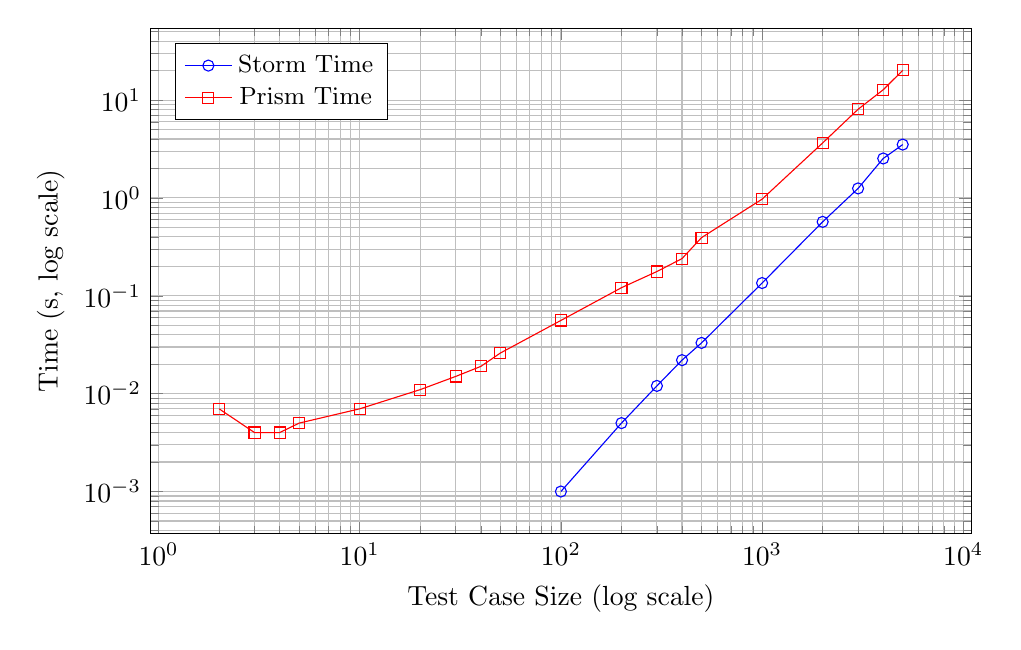
\begin{tikzpicture}
    \begin{loglogaxis}[
        width=12cm, height=8cm,
        xlabel={Test Case Size (log scale)},
        ylabel={Time (s, log scale)},
        grid=both,
        legend pos=north west,
        legend style={font=\small}
    ]
        % Storm Time Data
        \addplot+[mark=o, blue] coordinates {
            (100, 0.001)
            (200, 0.005)
            (300, 0.012)
            (400, 0.022)
            (500, 0.033)
            (1000, 0.135)
            (2000, 0.57)
            (3000, 1.251)
            (4000, 2.531)
            (5000, 3.511)
        };
        \addlegendentry{Storm Time}

        % Prism Time Data
        \addplot+[mark=square, red] coordinates {
            (2, 0.007)
            (3, 0.004)
            (4, 0.004)
            (5, 0.005)
            (10, 0.007)
            (20, 0.011)
            (30, 0.015)
            (40, 0.019)
            (50, 0.026)
            (100, 0.056)
            (200, 0.121)
            (300, 0.177)
            (400, 0.240)
            (500, 0.393)
            (1000, 0.972)
            (2000, 3.648)
            (3000, 8.057)
            (4000, 12.75)
            (5000, 20.134)
        };
        \addlegendentry{Prism Time}
    \end{loglogaxis}
\end{tikzpicture}
\caption{Log-Log Plot of Storm and Prism Runtimes}
\label{fig:loglog_runtime}
\end{figure}